\chapter{Детекция аномалий и анализ результатов}

\section{Постановка эксперимента для региональной модели}

В региональном эксперименте целью является не только получение прогнозного поля осадков, но и оценка способности модели детектировать экстремальные осадки как аномальные события. Для этого прогнозируемые суммы осадков сравниваются с картами порогов \(q_{0.9}\), после чего вычисляются вероятности и событийные метрики. Важное отличие от станционной части состоит в том, что здесь оценка производится по всему пространственному полю с учетом взвешивания по площади и региональных масок.

В этой главе приведены результаты нового ноутбука с моделью Earthformer-M. Визуализации получены из сохраненных артефактов лучшего запуска на сетке \(0.25^\circ\); для вставки в текст они приведены с русскими подписями, чтобы оформление было единообразным.

\section{Динамика обучения}

Первой важной характеристикой является стабильность обучения. По графику истории видно, что общий train loss уменьшается примерно с \(1.28\) на первой эпохе до \(0.61\) к двенадцатой эпохе. Это означает, что оптимизация остается устойчивой и не проявляет признаков численной неустойчивости. Это согласуется и с дополнительными проверками на \texttt{NaN}/\texttt{Inf}, встроенными в алгоритм: параметры и предсказания оставались конечными.

Для событийной постановки важнее не только значение функции потерь, но и якорная метрика ROCSS. На сетке \(0.25^\circ\) средний ROCSS по горизонтам 72, 120 и 240 часов сначала растет с уровня около \(0.17\), затем выходит на плато около \(0.24\)--\(0.26\). Максимум на графике достигается приблизительно на девятой эпохе. На дополнительной оценке \(1.5^\circ\) значения заметно ниже и находятся около \(0.03\)--\(0.06\), что показывает чувствительность результата к протоколу оценки и разрешению.

\begin{figure}[H]
    \centering
    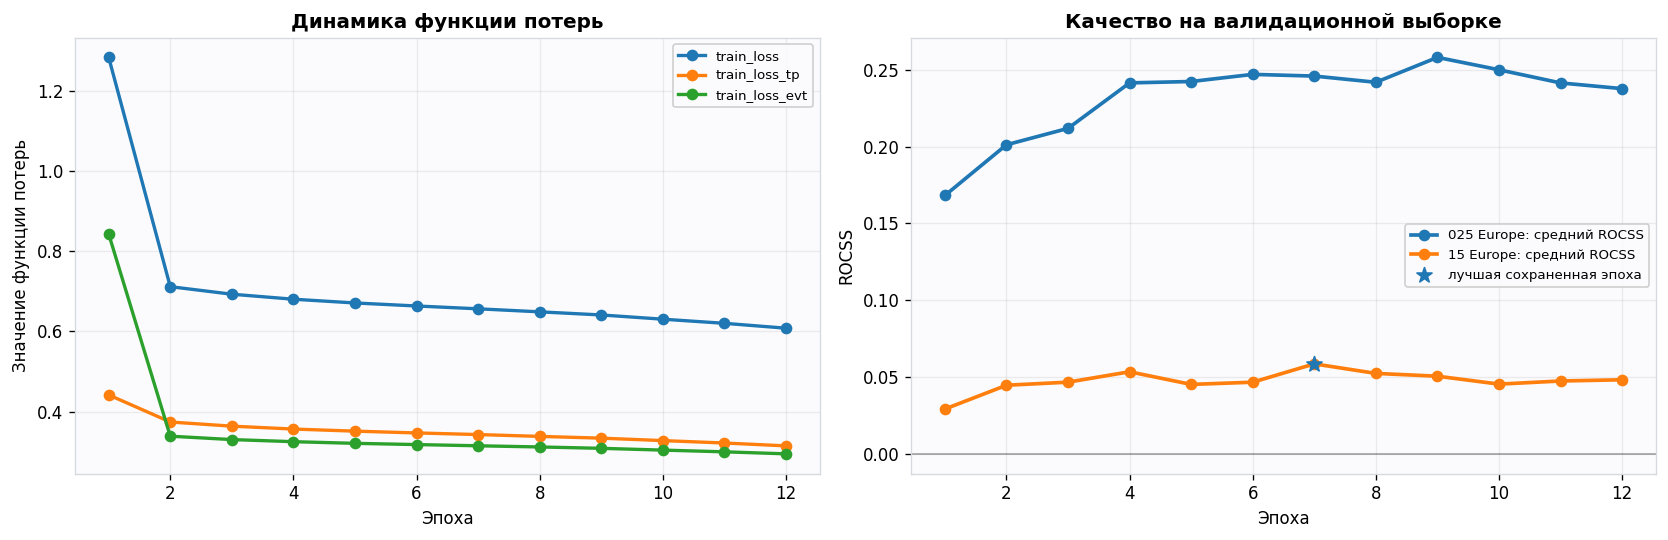
\includegraphics[width=0.95\textwidth]{figures/notebook/01_training_overview.png}
    \caption{Динамика обучения региональной модели Earthformer-M: изменение функции потерь и валидационной skill-метрики по эпохам.}
    \label{fig:training-overview}
\end{figure}

График на рисунке~\ref{fig:training-overview} удобен тем, что показывает не только численное снижение функции потерь, но и момент насыщения событийного качества. По нему видно, что уменьшение функции потерь продолжается, однако выигрыш по якорной метрике после первых эпох становится ограниченным. Поэтому дальше я рассматриваю не только значение функции потерь, но и набор специальных метрик для редких событий.

\begin{table}[H]
\centering
\begin{tabular}{cccc}
Эпоха & Train loss & ROCSS 0.25 Europe & ROCSS 1.5 Europe \\
1 & \(\approx 1.28\) & \(\approx 0.17\) & \(\approx 0.03\) \\
4 & \(\approx 0.68\) & \(\approx 0.24\) & \(\approx 0.05\) \\
7 & \(\approx 0.65\) & \(\approx 0.25\) & \(\approx 0.06\) \\
9 & \(\approx 0.64\) & \(\approx 0.26\) & \(\approx 0.05\) \\
12 & \(\approx 0.61\) & \(\approx 0.24\) & \(\approx 0.05\) \\
\end{tabular}
\caption{Динамика якорной метрики по истории нового запуска; значения восстановлены по графику и округлены}
\label{tab:anchor-rocss}
\end{table}

Содержательно таблица~\ref{tab:anchor-rocss} показывает, что оптимальное качество по событийной метрике достигается раньше, чем минимальное значение функции потерь. Это типичная ситуация для задач с редкими событиями: дальнейшее улучшение общей функции потерь не обязательно улучшает качество по экстремумам. Следовательно, для отбора лучшего чекпоинта необходимо ориентироваться именно на вероятностные метрики редких событий, а не только на обобщенную функцию потерь.

\section{Качество детекции экстремальных осадков на нативной сетке}

Наиболее содержательными для интерпретации являются метрики на конкретных горизонтах. В новом запуске модель очень сильна на ближайшем горизонте 24 часа: для Европы ROC-AUC равен \(0.9017\), ROCSS равен \(0.8034\), PR-AUC равен \(0.4065\). После этого качество быстро снижается с ростом горизонта прогноза. На горизонтах 72, 120 и 240 часов ROCSS остается положительным, но уже находится на уровнях \(0.3287\), \(0.2352\) и \(0.1738\) соответственно.

\begin{figure}[H]
    \centering
    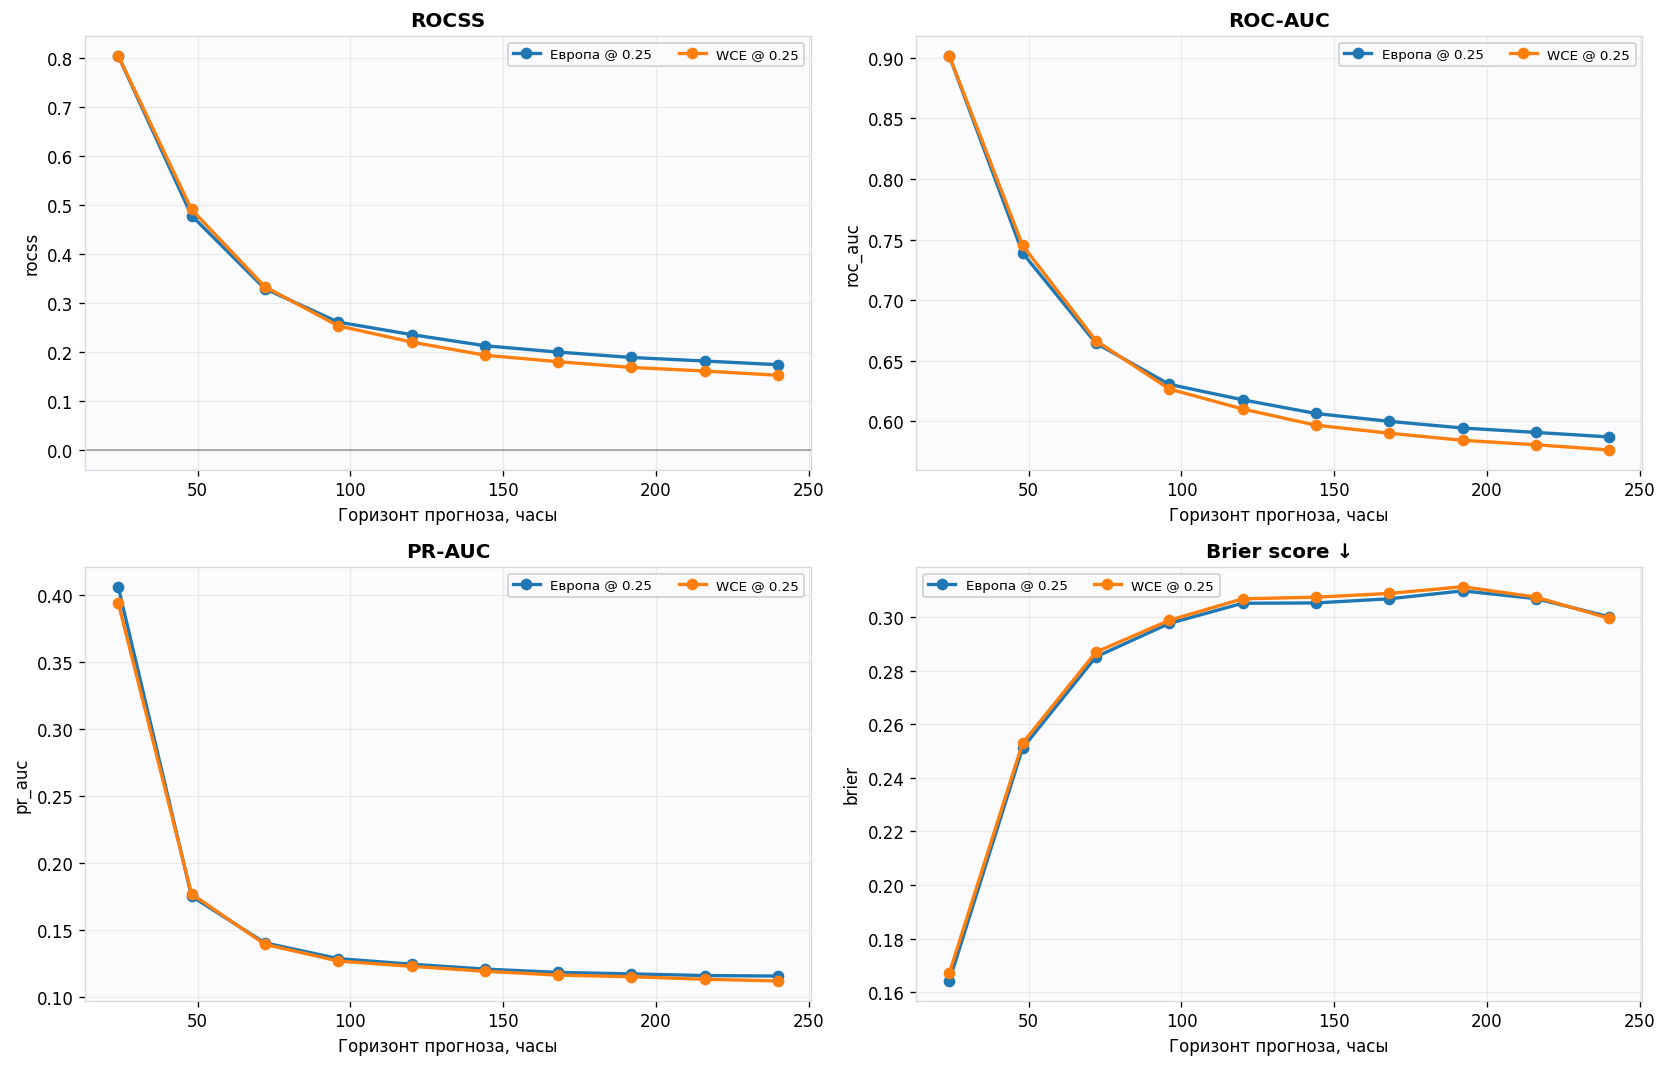
\includegraphics[width=0.98\textwidth]{figures/notebook/02_metrics_by_lead.png}
    \caption{Зависимость основных вероятностных метрик от горизонта прогноза. На графике собраны ROCSS, ROC-AUC, PR-AUC и Brier score для разных горизонтов прогноза.}
    \label{fig:metrics-by-lead}
\end{figure}

Рисунок~\ref{fig:metrics-by-lead} хорошо иллюстрирует резкую деградацию качества после первых суток. Для осадков это ожидаемо, поскольку поле осадков имеет высокую пространственную неоднородность и сильную зависимость от синоптической ситуации. При этом важное отличие нового запуска состоит в том, что Brier score на средних и дальних горизонтах заметно ухудшается и держится около \(0.30\). Это указывает, что модель сохраняет некоторую способность ранжировать риск, но вероятности требуют дополнительной калибровки.

\begin{table}[H]
\centering
\begin{tabular}{ccccc}
Горизонт & ROCSS & ROC-AUC & PR-AUC & Brier \\
24 ч & 0.8034 & 0.9017 & 0.4065 & 0.1642 \\
72 ч & 0.3287 & 0.6644 & 0.1405 & 0.2851 \\
120 ч & 0.2352 & 0.6176 & 0.1246 & 0.3051 \\
240 ч & 0.1738 & 0.5869 & 0.1157 & 0.3001 \\
\end{tabular}
\caption{Итоговые метрики для региона Europe на сетке \(0.25^\circ\) по новому ноутбуку}
\label{tab:best-025}
\end{table}

При интерпретации таблицы~\ref{tab:best-025} важно обратить внимание на два обстоятельства.

Во-первых, skill закономерно убывает с ростом горизонта прогноза. На 24 часах модель очень хорошо различает экстремальные и неэкстремальные случаи, на 72 часах качество остается полезным, а к 240 часам заметно снижается. Такая деградация ожидаема из-за накопления ошибки и ограниченной предсказуемости атмосферных процессов. Однако даже на 240 часах ROCSS остается положительным, что свидетельствует о сохранении некоторой прогностической информации.

Во-вторых, PR-AUC по абсолютному значению после 48 часов невелика. Это не является признаком \enquote{плохой модели} само по себе; в задачах экстремальных событий с редким положительным классом низкие значения PR-AUC типичны. Здесь важно сравнение не с абсолютной шкалой \([0,1]\), а с базовой частотой события. В то же время высокий Brier score показывает, что вероятности в новом запуске нельзя напрямую трактовать как хорошо откалиброванные.

\section{Сравнение станционных и сеточных результатов}

Хотя две части работы нельзя сравнивать напрямую \enquote{число к числу} из-за различия данных, объектов и протоколов оценки, сопоставление общих закономерностей оказывается информативным.

В станционной части лучшими оказались бустинговые модели, причем XGBoost достиг среднего ROCSS \(0.4469\) на валидации, а на горизонте 24 часа показал ROCSS \(0.3809\). В новом сеточном запуске на горизонте 24 часа ROCSS выше, но на средних и дальних горизонтах значения оказываются ниже станционного среднего. Такое сопоставление не следует интерпретировать как прямое превосходство одной постановки над другой: станционная модель решает более локальную задачу, а сеточная модель прогнозирует полное поле, несколько горизонтов и несколько ансамблевых членов.

В сеточной части глубокая модель работает в существенно более сложной постановке. Она прогнозирует полное пространственное поле, несколько горизонтов прогноза и несколько ансамблевых членов. Поэтому более низкие значения метрик на дальних горизонтах сами по себе не означают меньшую ценность подхода. Именно глубокая модель делает возможными задачи, которые станционная базовая модель решить не может: пространственно-согласованный прогноз, детекцию аномалий по картам квантилей и анализ пространственной структуры ошибок.

\begin{figure}[H]
    \centering
    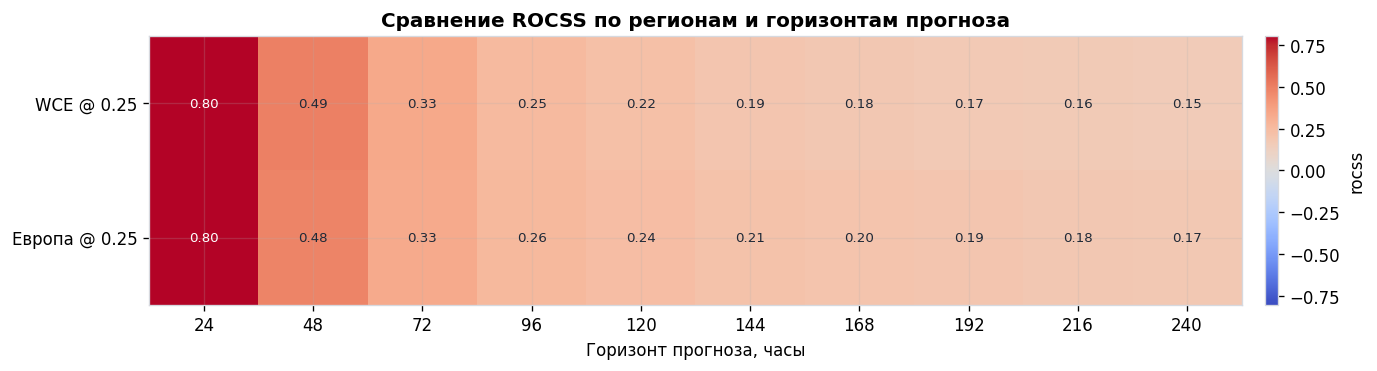
\includegraphics[width=0.90\textwidth]{figures/notebook/03_rocss_heatmap.png}
    \caption{Сравнение ROCSS по регионам и горизонтам прогноза. Тепловая карта показывает, как меняется качество при увеличении горизонта прогноза.}
    \label{fig:rocss-heatmap}
\end{figure}

\begin{figure}[H]
    \centering
    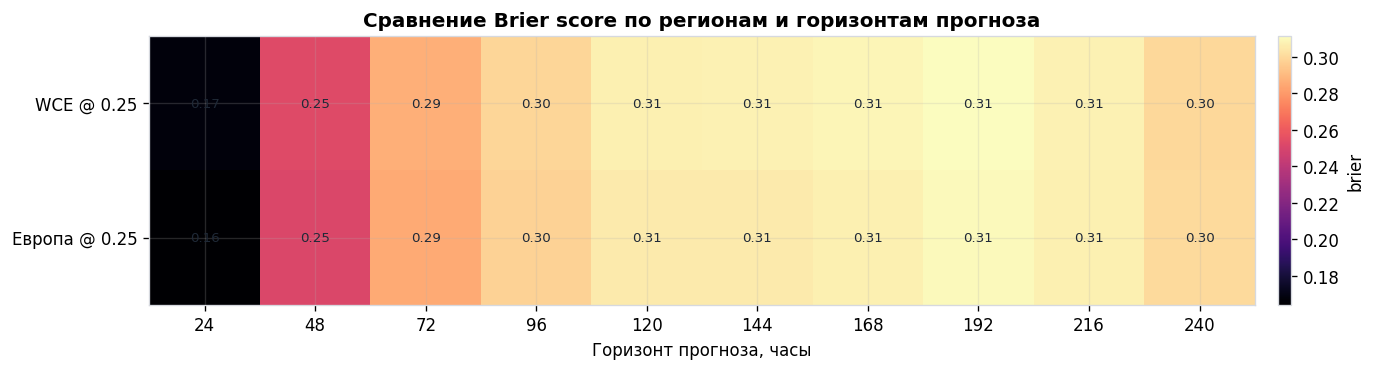
\includegraphics[width=0.90\textwidth]{figures/notebook/04_brier_heatmap.png}
    \caption{Сравнение Brier score по регионам и горизонтам прогноза. Эта метрика дополняет ROCSS, так как учитывает не только ранжирование событий, но и численное качество вероятностей.}
    \label{fig:brier-heatmap}
\end{figure}

На рисунках~\ref{fig:rocss-heatmap} и~\ref{fig:brier-heatmap} видно, что качество нельзя описать одной итоговой цифрой. Оно меняется по регионам и по горизонтам прогноза, причем дальние горизонты ожидаемо оказываются сложнее. Поэтому я рассматриваю набор метрик вместе, а не ограничиваюсь только одним показателем.

Если сформулировать вывод аккуратно, он звучит так: \textit{станционные бустинги являются сильной и обязательной базовой моделью для локального прогноза, но глубокие нейросетевые модели необходимы в тех случаях, когда задача требует явной пространственной структуры и многогоризонтного сеточного прогноза.} Таким образом, две части работы не противоречат друг другу, а образуют логическую иерархию сложности.

\section{Детекция аномалий как самостоятельная задача}

Один из главных содержательных результатов работы состоит в том, что детекция аномалий в климатических данных может быть естественно интегрирована в прогнозную модель, а не рассматриваться как отдельный постобработочный этап. Это видно на обоих уровнях:
\begin{itemize}
    \item в станционной постановке аномалия определяется через превышение \(q_{0.9}\) и вероятность вычисляется из регрессионного прогноза;
    \item в сеточной постановке аномалия поддерживается через вспомогательную головную часть события и через вероятностную интерпретацию прогноза осадков.
\end{itemize}

Такой подход имеет несколько преимуществ. Во-первых, модель обучается на физически интерпретируемой величине — сумме осадков — и не теряет связи с основной метеорологической задачей. Во-вторых, вероятностная детекция строится на том же скрытом представлении, что и прогноз, а значит, использует максимально богатую информацию. В-третьих, это позволяет варьировать порог экстремальности без полного переобучения модели, если требуется перейти от \(q_{0.9}\) к более жесткому или более мягкому критерию.

\begin{figure}[H]
    \centering
    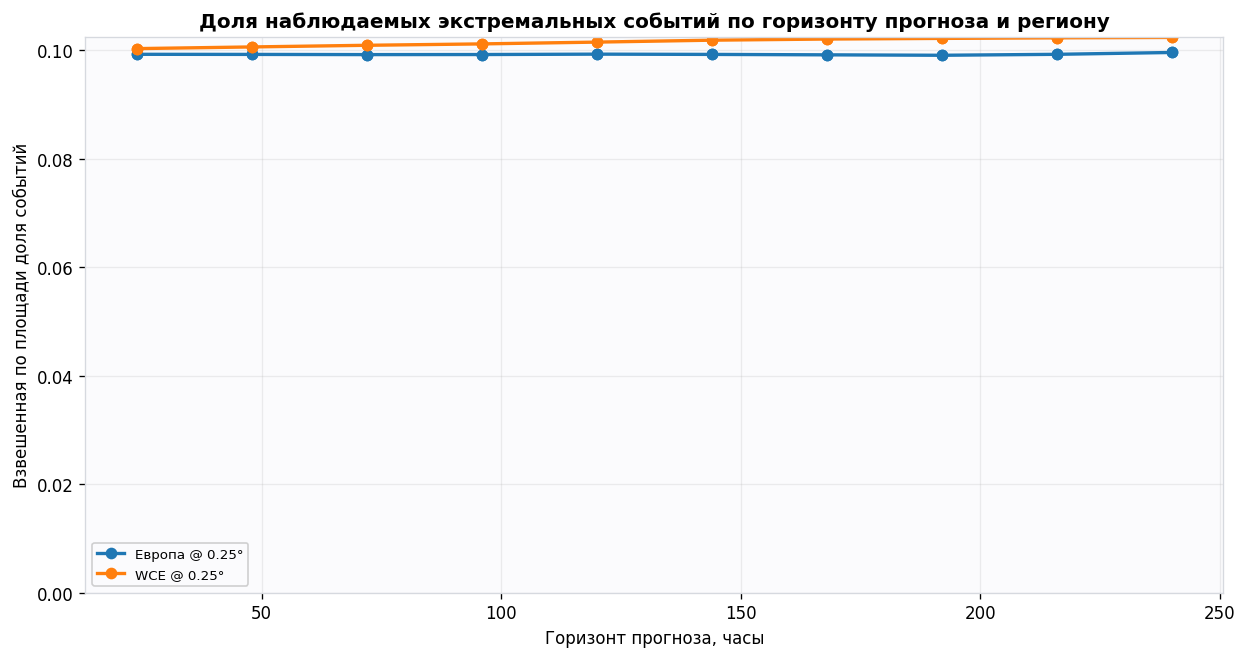
\includegraphics[width=0.95\textwidth]{figures/notebook/16_event_rate_by_lead_region_grid.png}
    \caption{Доля наблюдаемых экстремальных событий по горизонту прогноза и региону. График показывает базовую частоту положительного класса, относительно которой следует интерпретировать PR-AUC и метрики таблицы сопряженности.}
    \label{fig:event-rate-by-lead}
\end{figure}

На рисунке~\ref{fig:event-rate-by-lead} показана базовая частота события. В новом запуске она остается близкой к ожидаемым \(10\%\): для Европы значения составляют примерно \(0.099\) на всех горизонтах, а для Западной и Центральной Европы — около \(0.100\)--\(0.102\). Этот график важен, потому что без него легко неверно интерпретировать PR-AUC: при редком положительном классе даже умеренные абсолютные значения PR-AUC могут означать заметный выигрыш относительно климатологического уровня.

\begin{figure}[H]
    \centering
    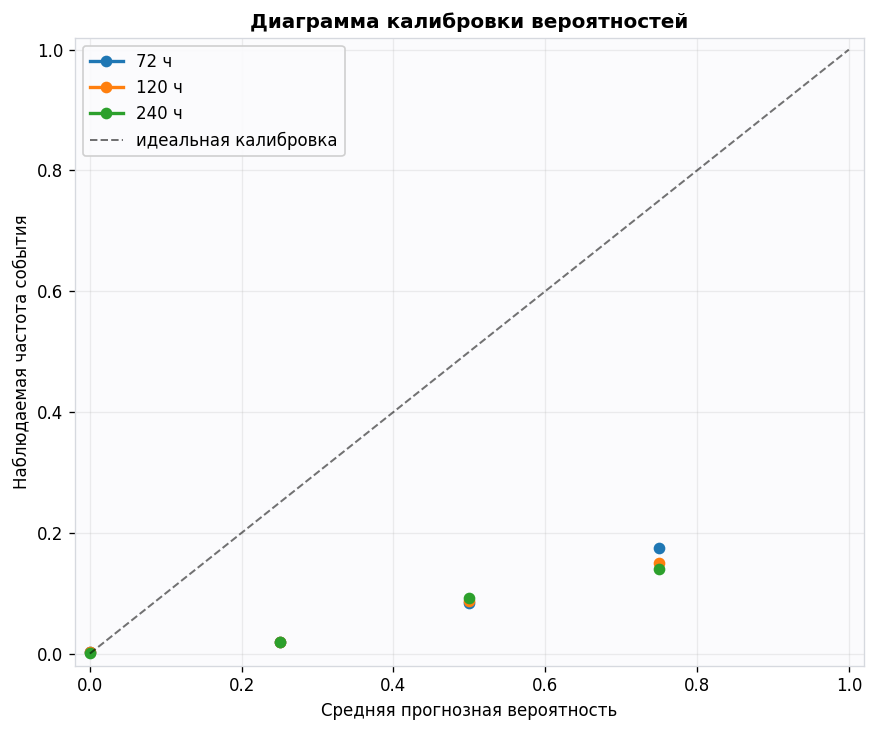
\includegraphics[width=0.82\textwidth]{figures/notebook/05_reliability_europe.png}
    \caption{Диаграмма надежности для вероятностной детекции экстремальных осадков. Она сравнивает предсказанные вероятности с фактическими частотами событий.}
    \label{fig:reliability-europe}
\end{figure}

\begin{figure}[H]
    \centering
    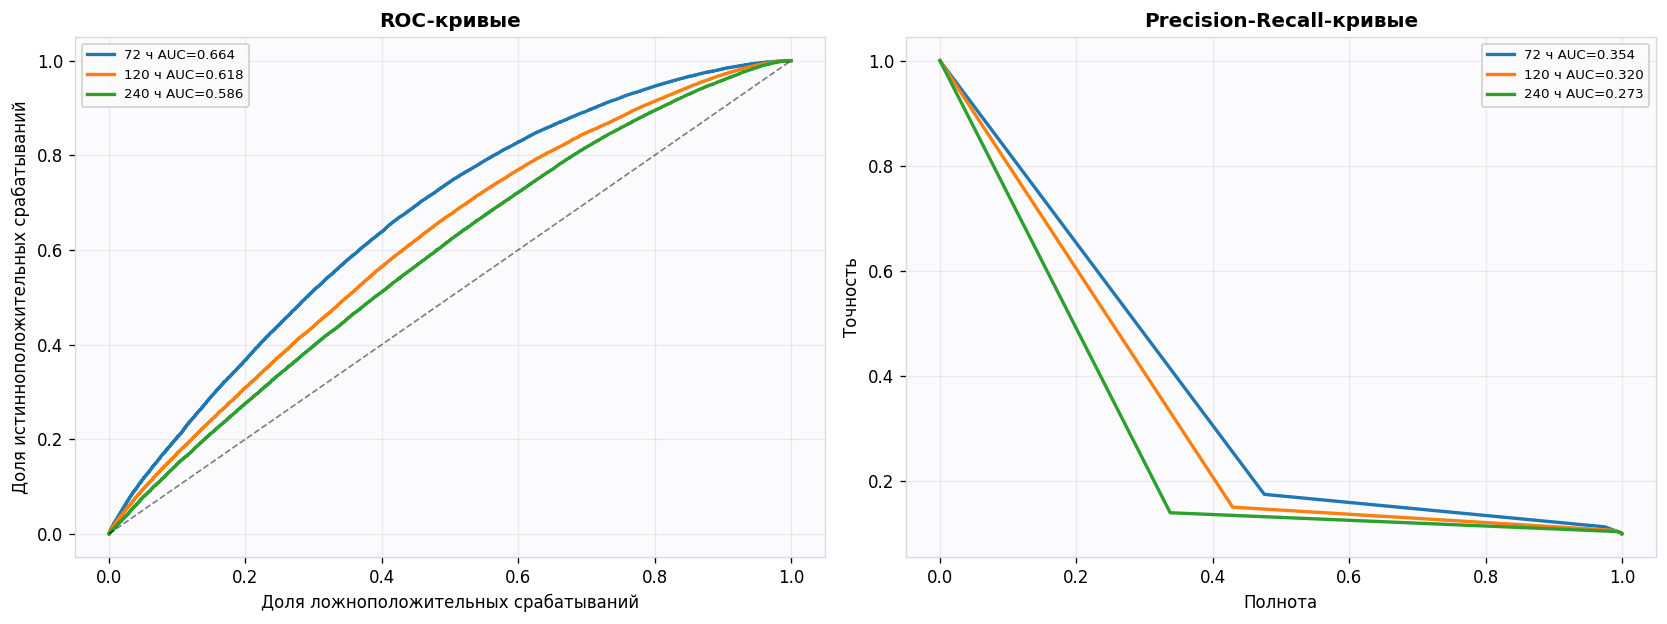
\includegraphics[width=0.95\textwidth]{figures/notebook/06_roc_pr_curves_europe.png}
    \caption{ROC- и PR-кривые для Европы. ROC-кривая показывает качество ранжирования, а PR-кривая особенно важна из-за редкости экстремальных событий.}
    \label{fig:roc-pr-europe}
\end{figure}

Рисунки~\ref{fig:reliability-europe} и~\ref{fig:roc-pr-europe} разделяют две разные стороны вероятностного прогноза. ROC/PR-кривые отвечают на вопрос, насколько хорошо модель ранжирует опасные случаи относительно обычных, а reliability diagram показывает, можно ли напрямую трактовать значения как откалиброванные вероятности. В новом запуске точки reliability diagram лежат существенно ниже диагонали идеальной калибровки, то есть модель переоценивает вероятность события. Для практического использования это различие существенно: модель может быть полезной для ранжирования риска, но при этом требовать дополнительной калибровки вероятностей.

\begin{figure}[p]
    \centering
    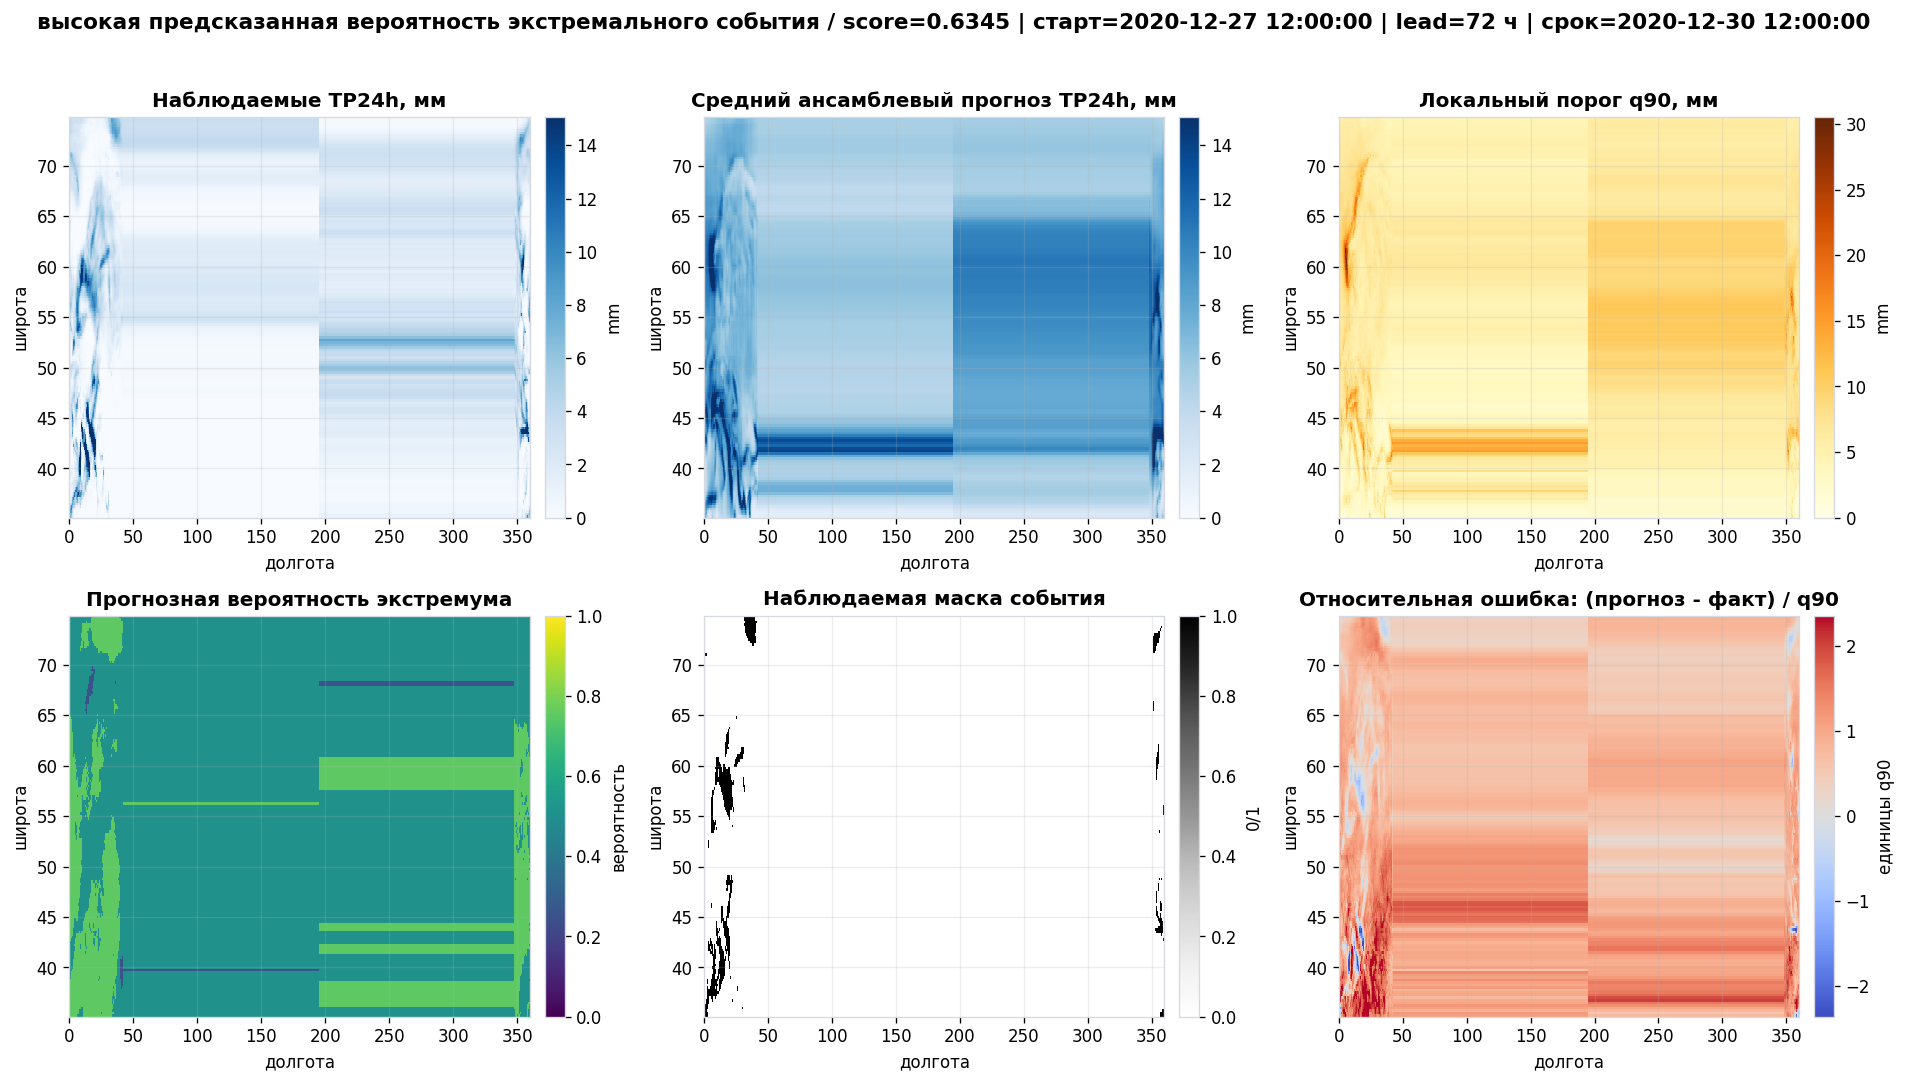
\includegraphics[width=\textwidth]{figures/notebook/08_case_max_prob_72h.png}
    \caption{Пример пространственного прогноза для случая с высокой предсказанной вероятностью экстремального события на горизонте 72 часа. Панели показывают наблюдаемые осадки, прогноз, локальный порог, вероятность события и маску фактического превышения.}
    \label{fig:case-max-prob-72}
\end{figure}

\begin{figure}[p]
    \centering
    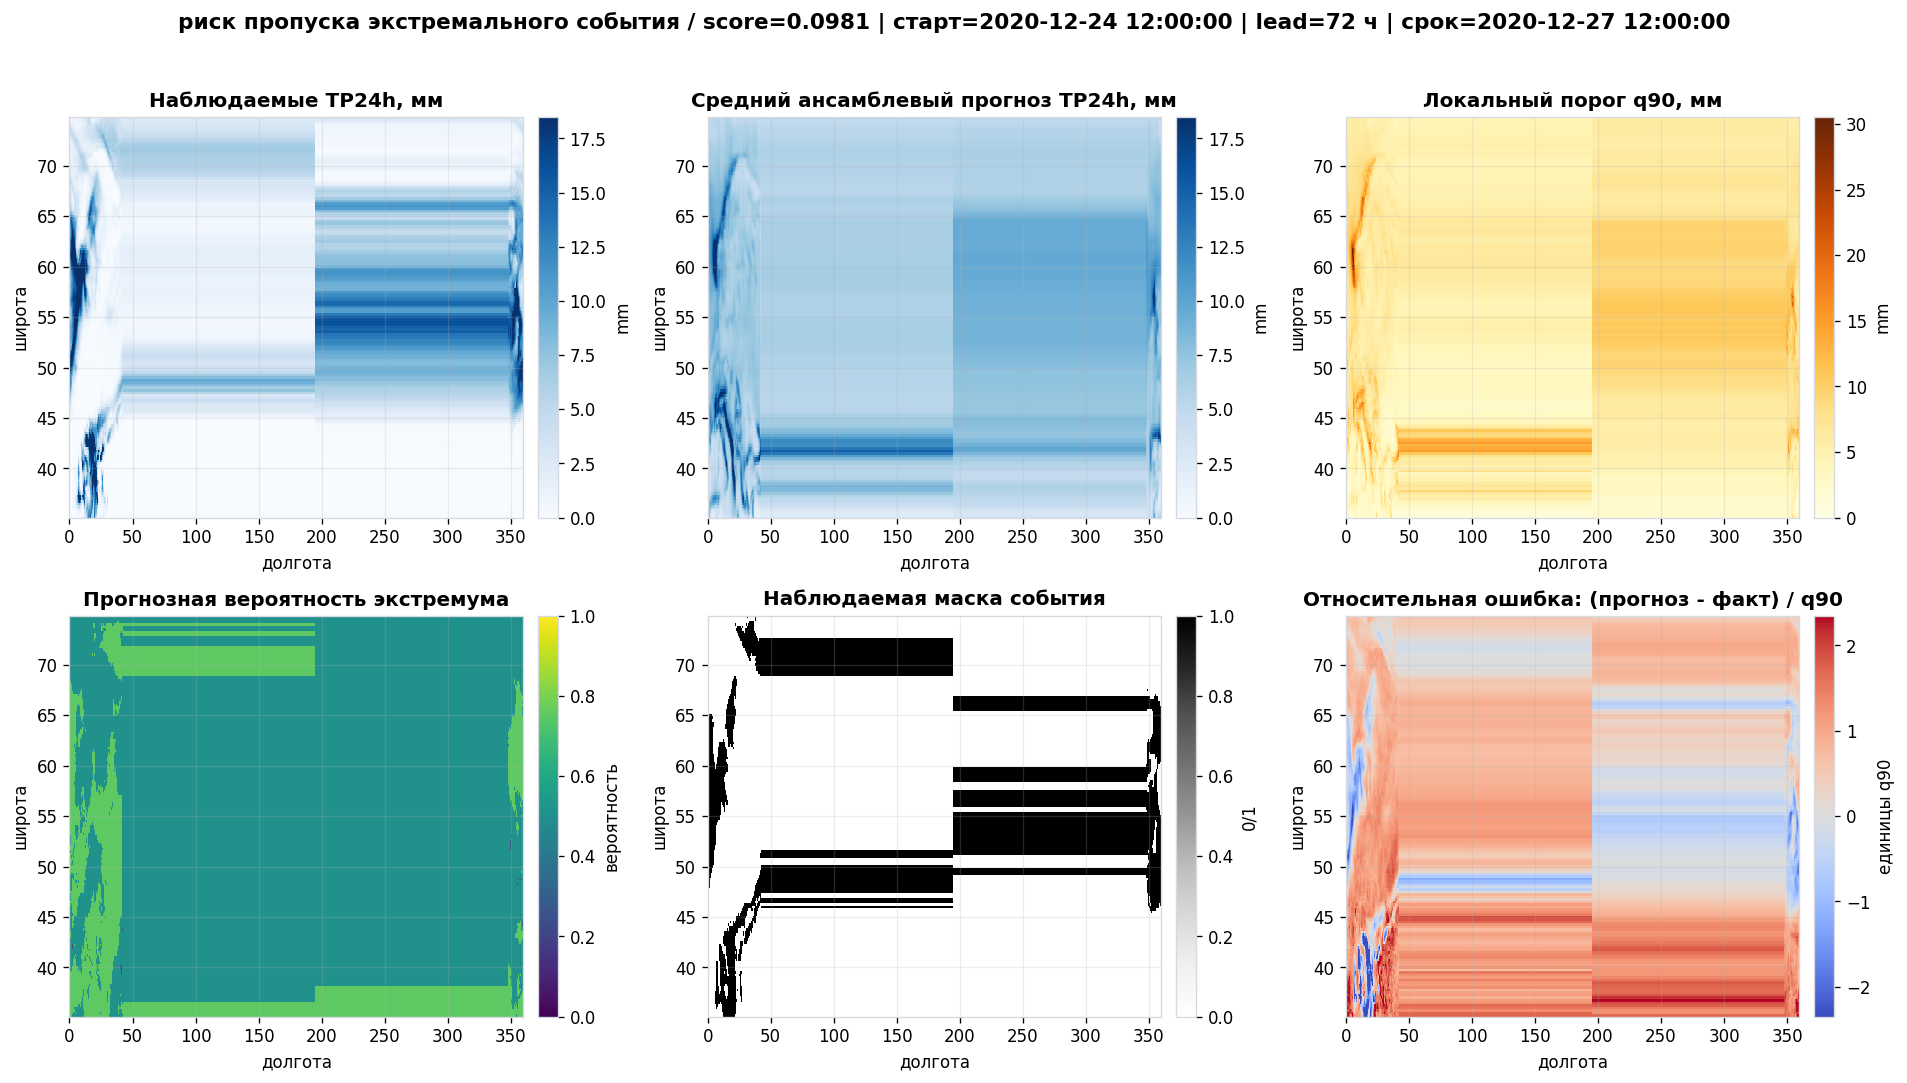
\includegraphics[width=\textwidth]{figures/notebook/08_case_miss_risk_72h.png}
    \caption{Пример случая с риском пропуска экстремального события на горизонте 72 часа. Такой пример полезен для анализа не только успешных прогнозов, но и типичных ограничений модели.}
    \label{fig:case-miss-risk-72}
\end{figure}

Пространственные примеры на рисунках~\ref{fig:case-max-prob-72} и~\ref{fig:case-miss-risk-72} нужны не для замены численных метрик, а для проверки их содержательного смысла. По ним видно, где модель улавливает область повышенного риска, а где вероятностный прогноз может быть слишком сглаженным или смещенным относительно фактического пятна осадков. Для меня это важная часть анализа, потому что в сеточной задаче качество поля нельзя полностью описать одной усредненной метрикой.

С прикладной точки зрения это особенно важно для систем раннего предупреждения. Операционному пользователю часто нужны не только \enquote{ожидаемые миллиметры осадков}, но и вероятность того, что будет превышен определенный опасный уровень. Архитектура, одновременно поддерживающая обе интерпретации, оказывается гораздо полезнее детерминированного прогноза без оценки риска.

\section{Калибровка, смещение вероятностей и неопределенность}

Помимо threshold-free метрик, таких как ROC-AUC и PR-AUC, необходимо отдельно анализировать калибровку вероятностей. В новом запуске именно калибровка является главным ограничением: средняя предсказанная вероятность события оказывается намного выше фактической частоты события.

\begin{figure}[H]
    \centering
    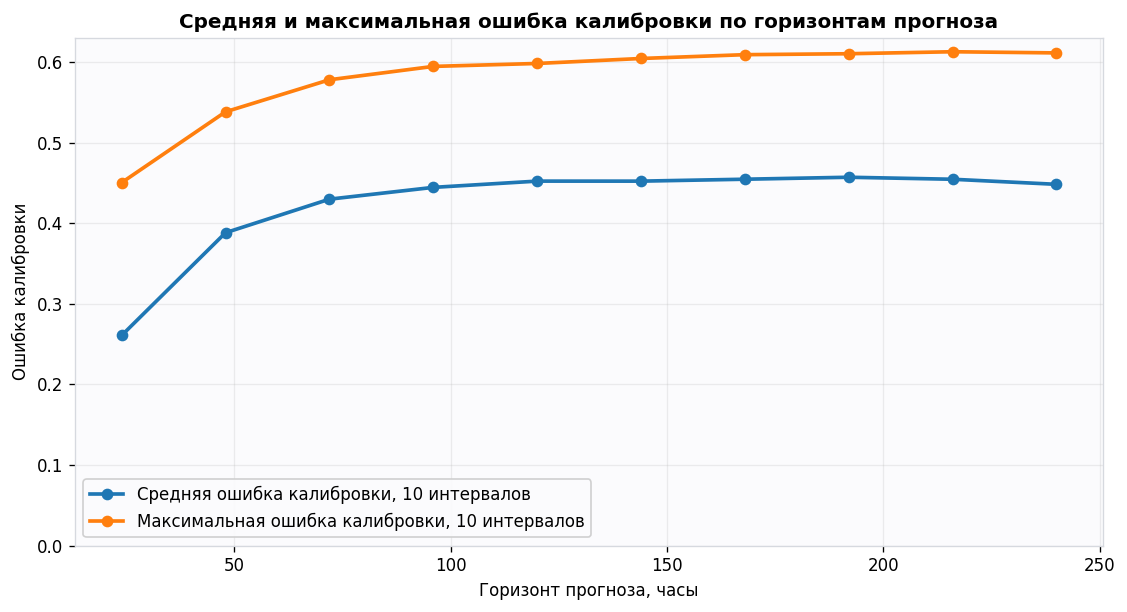
\includegraphics[width=0.86\textwidth]{figures/notebook/17_calibration_error_by_lead_europe.png}
    \caption{Средняя ошибка калибровки и максимальная ошибка калибровки по горизонтам прогноза для Европы.}
    \label{fig:calibration-error}
\end{figure}

\begin{figure}[H]
    \centering
    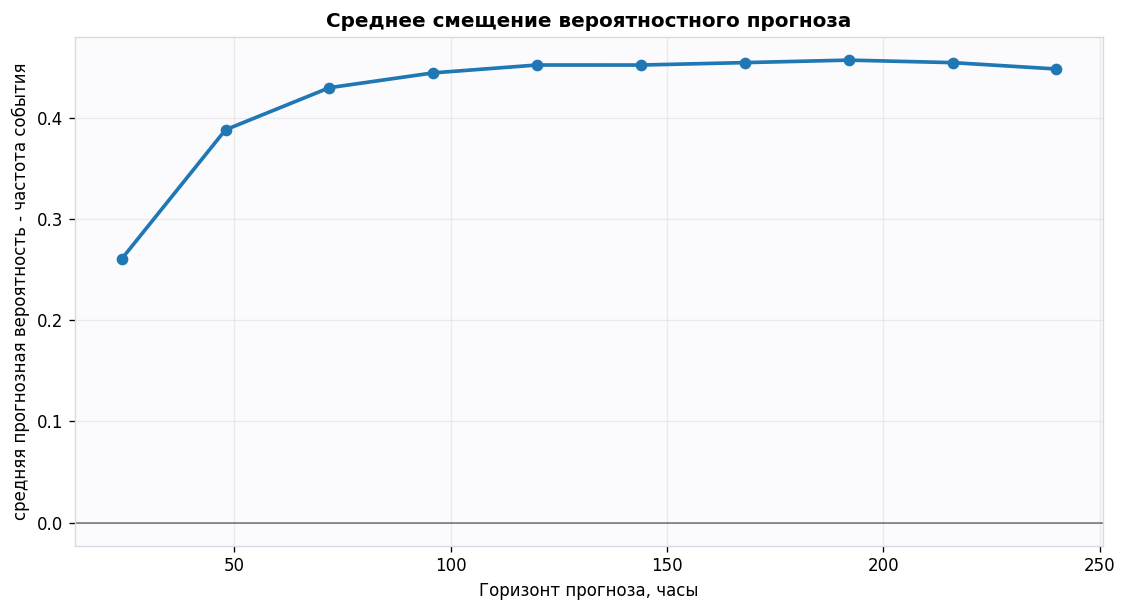
\includegraphics[width=0.86\textwidth]{figures/notebook/18_probability_bias_by_lead_europe.png}
    \caption{Среднее смещение вероятностного прогноза: разность между средней предсказанной вероятностью и фактической частотой события.}
    \label{fig:probability-bias}
\end{figure}

\begin{table}[H]
\centering
\begin{tabular}{ccccc}
Горизонт & ECE & MCE & Средняя вероятность & Частота события \\
24 ч & 0.2608 & 0.4503 & 0.3597 & 0.0992 \\
72 ч & 0.4297 & 0.5778 & 0.5288 & 0.0991 \\
120 ч & 0.4521 & 0.5980 & 0.5516 & 0.0996 \\
240 ч & 0.4482 & 0.6111 & 0.5471 & 0.0990 \\
\end{tabular}
\caption{Калибровочные показатели для региона Europe на сетке \(0.25^\circ\)}
\label{tab:calibration-025}
\end{table}

Рисунки~\ref{fig:calibration-error} и~\ref{fig:probability-bias}, а также таблица~\ref{tab:calibration-025}, показывают, что вероятностный выход модели следует анализировать отдельно от качества ранжирования. Даже если ROC-AUC остается положительным, вероятности могут быть систематически завышены. В данном запуске средняя прогнозная вероятность на горизонтах 72--240 часов находится около \(0.53\)--\(0.55\), тогда как фактическая частота события близка к \(0.10\). Поэтому при операционном использовании такой модели необходимо добавить калибровочный слой, например isotonic regression или temperature scaling на отдельной валидационной выборке.

\begin{figure}[H]
    \centering
    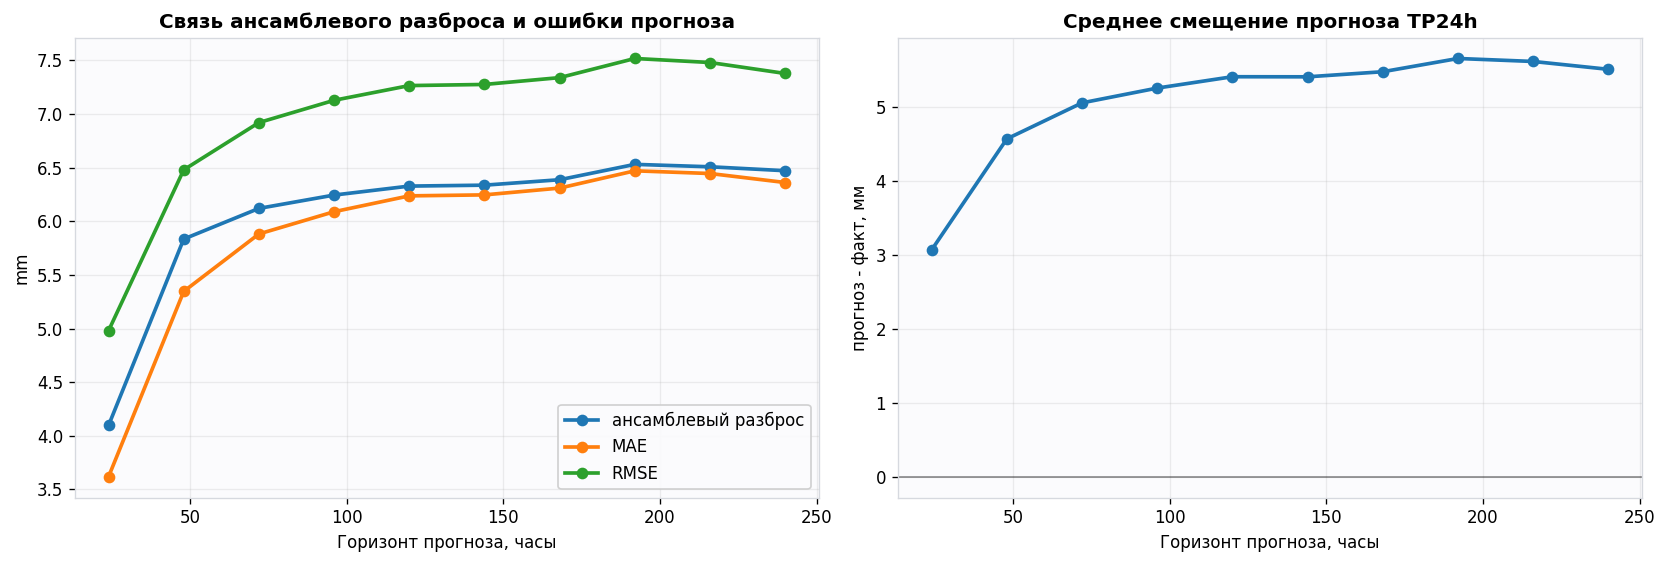
\includegraphics[width=0.92\textwidth]{figures/notebook/12_spread_error_by_lead.png}
    \caption{Связь ансамблевого разброса и ошибки прогноза по горизонту прогноза. График используется как простая проверка того, несет ли ансамбль информацию о неопределенности.}
    \label{fig:spread-error-by-lead}
\end{figure}

\begin{figure}[H]
    \centering
    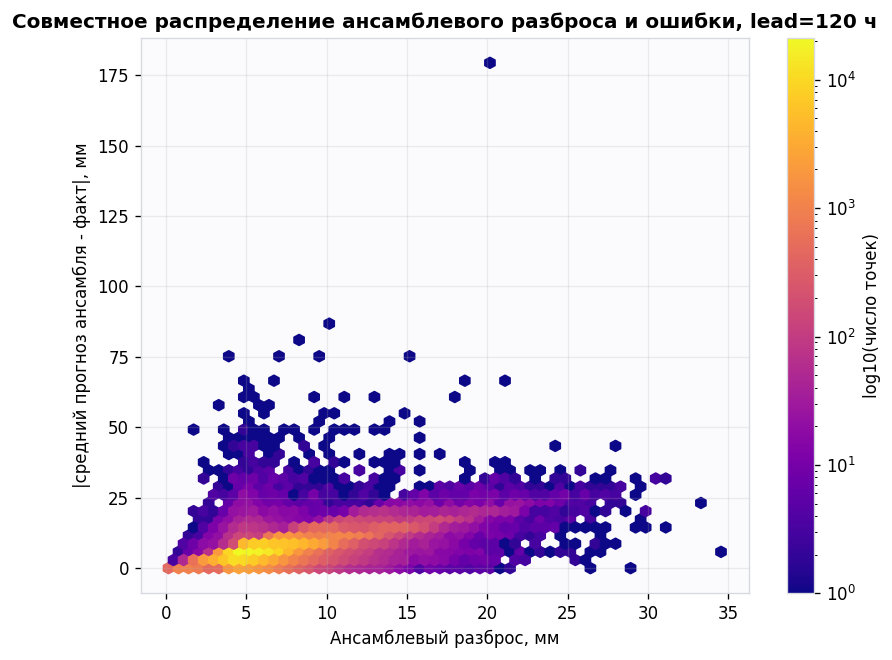
\includegraphics[width=0.92\textwidth]{figures/notebook/13_spread_error_hexbin_120h.png}
    \caption{Совместное распределение ансамблевого разброса и ошибки для горизонта 120 часов. Такой вид графика позволяет увидеть не только средний тренд, но и плотность отдельных случаев.}
    \label{fig:spread-error-hexbin}
\end{figure}

\begin{table}[H]
\centering
\begin{tabular}{ccccc}
Горизонт & Разброс, мм & MAE, мм & RMSE, мм & Bias, мм \\
24 ч & 4.10 & 3.62 & 4.98 & 3.06 \\
72 ч & 6.12 & 5.88 & 6.92 & 5.05 \\
120 ч & 6.33 & 6.24 & 7.26 & 5.40 \\
240 ч & 6.47 & 6.36 & 7.38 & 5.50 \\
\end{tabular}
\caption{Ансамблевый разброс и ошибки прогноза осадков по выбранным горизонтам}
\label{tab:spread-error-025}
\end{table}

Ансамблевая постановка нужна не только для усреднения прогноза, но и для оценки неопределенности. Рисунки~\ref{fig:spread-error-by-lead} и~\ref{fig:spread-error-hexbin} показывают, насколько ансамблевый разброс связан с фактической ошибкой. При этом таблица~\ref{tab:spread-error-025} выявляет еще одну особенность нового запуска: прогноз имеет выраженное положительное смещение по сумме осадков. Это согласуется с завышением вероятностей экстремального события и указывает, что модель склонна к переоценке влажных сценариев.

\begin{figure}[p]
    \centering
    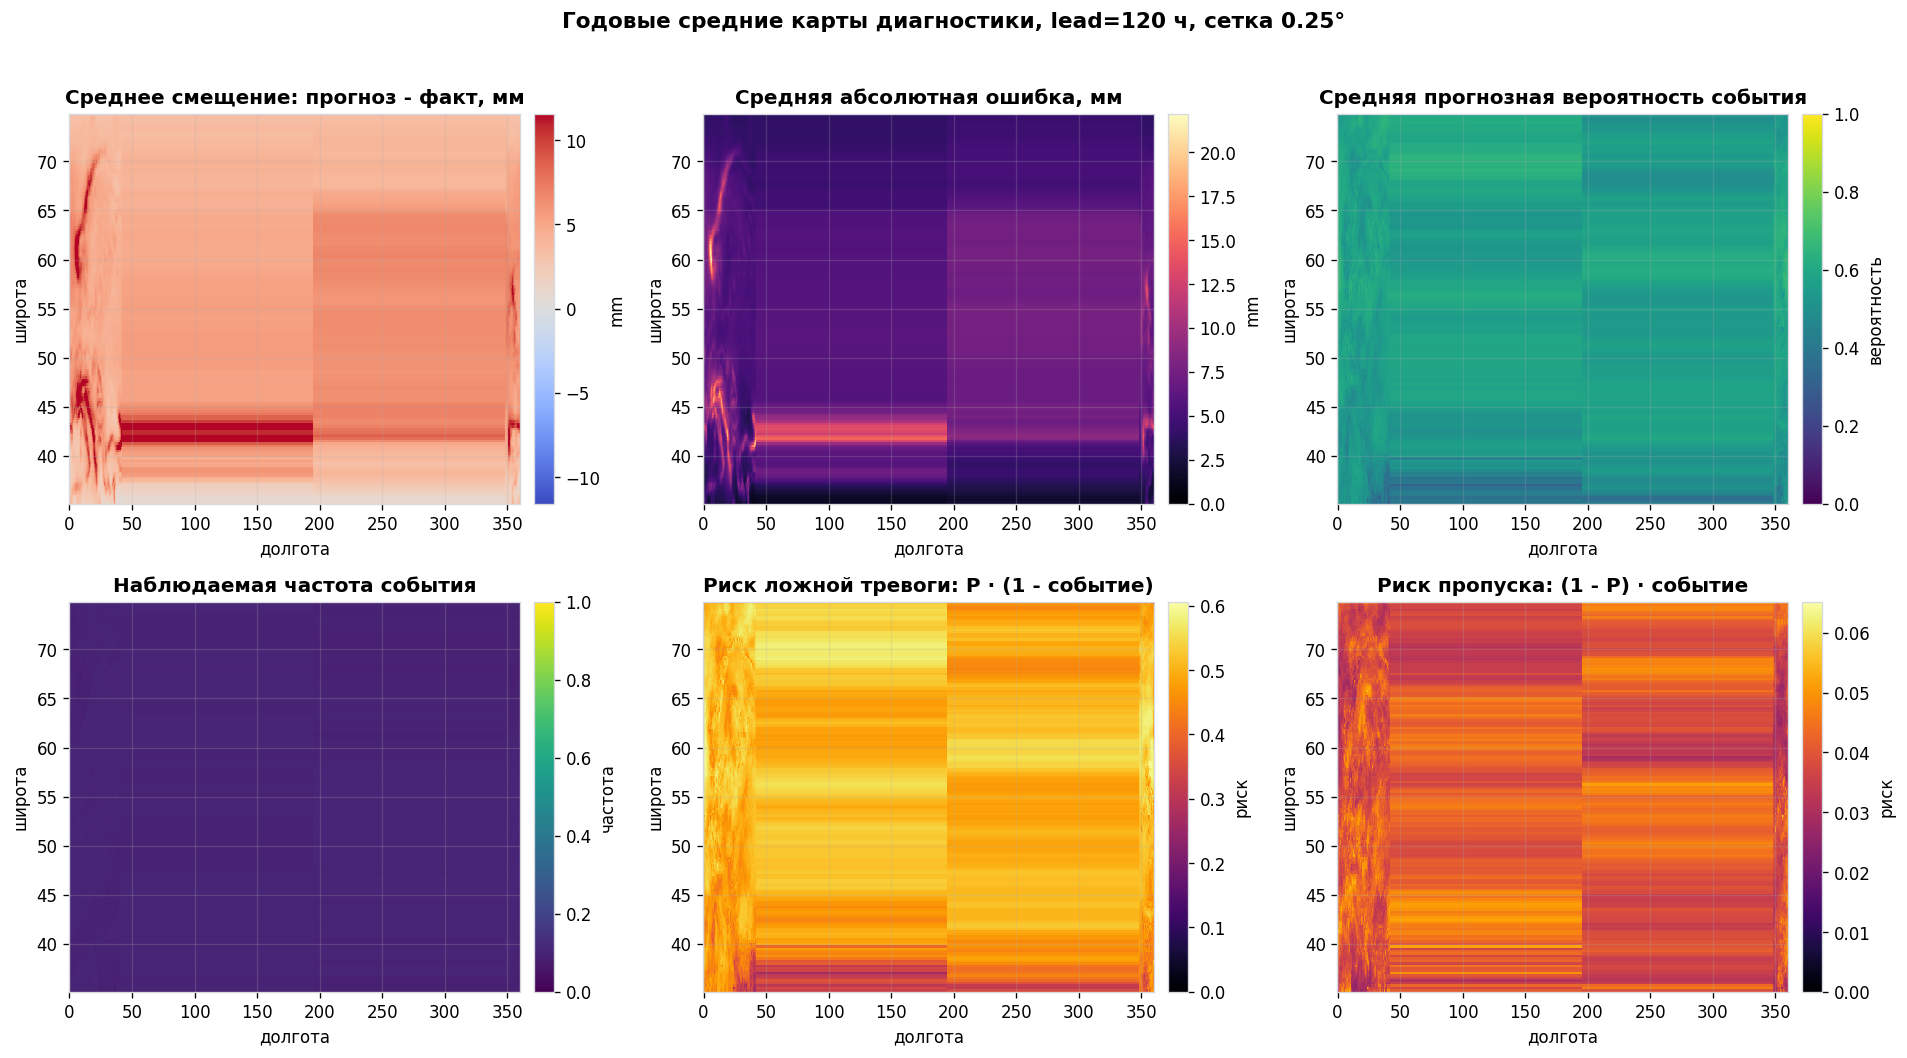
\includegraphics[width=\textwidth]{figures/notebook/14_year_mean_anomaly_maps_120h.png}
    \caption{Годовые средние карты диагностики на горизонте 120 часов: аномалия, ошибка, средняя вероятность события, частота события, false alarm rate и miss rate.}
    \label{fig:year-mean-anomaly-maps}
\end{figure}

\begin{figure}[H]
    \centering
    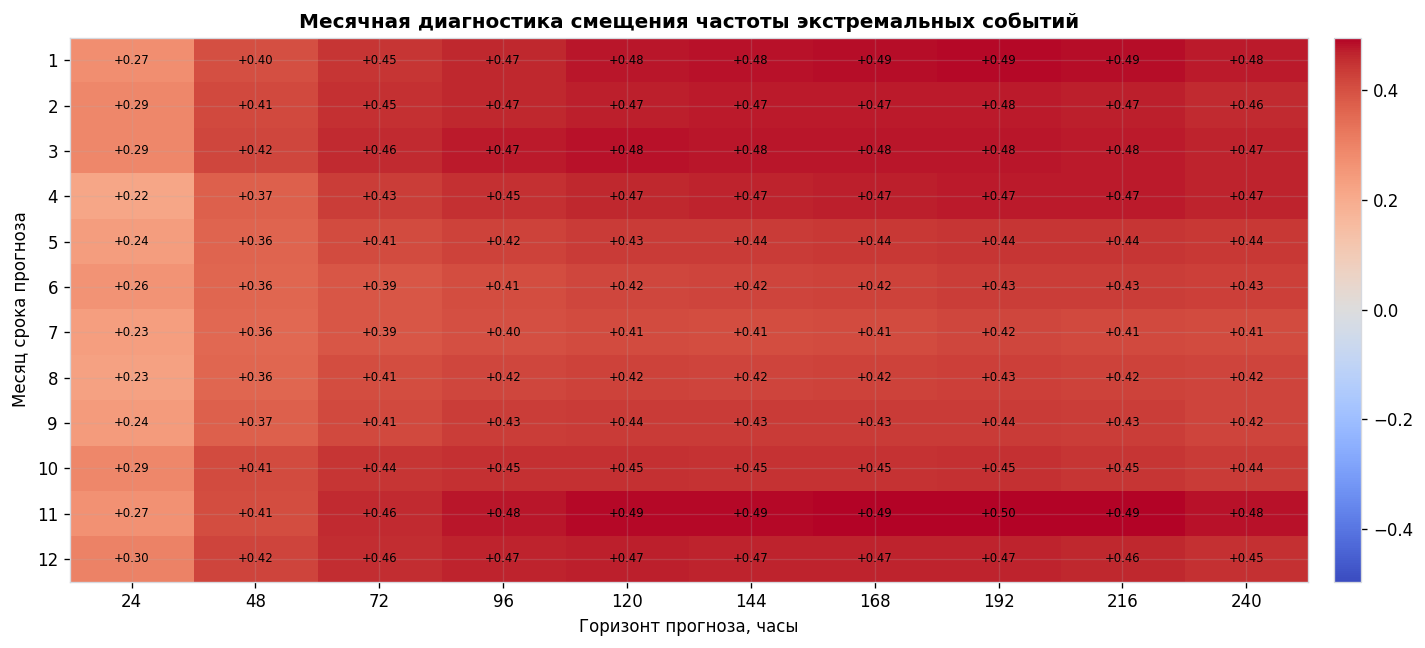
\includegraphics[width=0.95\textwidth]{figures/notebook/10_monthly_event_rate_bias.png}
    \caption{Месячная диагностика смещения частоты экстремальных событий. Рисунок показывает, что ошибки модели имеют не только пространственную, но и сезонную структуру.}
    \label{fig:monthly-event-rate-bias}
\end{figure}

Рисунки~\ref{fig:year-mean-anomaly-maps} и~\ref{fig:monthly-event-rate-bias} показывают, что ошибки модели неоднородны по пространству и сезону. Усредненная метрика может скрывать области с повышенной долей пропусков или ложных тревог, поэтому карты и месячные разрезы используются как отдельный источник информации о надежности прогноза.

\section{Выводы по экспериментальной части}

Результаты экспериментальной части можно свести к нескольким выводам.

Первый вывод состоит в том, что станционные табличные модели с богатой инженерией признаков являются сильной базовой моделью для локального прогноза осадков. В рамках доступных экспериментов наилучшей моделью оказался XGBoost, а климатология показала сильный результат на дальнем горизонте 240 часов.

Второй вывод связан с региональной нейросетевой моделью Earthformer-M. Она демонстрирует устойчивое обучение и очень высокое качество ранжирования на ближайшем горизонте 24 часа, однако на средних и дальних горизонтах skill заметно снижается. Тем не менее ROCSS остается положительным, то есть модель извлекает полезный пространственно-временной сигнал для детекции аномальных осадков.

Третий вывод относится к вероятностной постановке. Детекция аномалий в климатических данных естественно формулируется как прогноз редкого события превышения квантильного порога. Такая схема связывает регрессию и классификацию в одной экспериментальной процедуре.

Четвертый вывод касается практического применения. Полученные вероятности полезны для ранжирования риска, но в новом запуске они заметно завышены. Поэтому перед использованием в системе предупреждения необходимо выполнить отдельную калибровку вероятностей и затем выбирать порог вероятности с учетом цены пропуска и ложной тревоги.
